\section{Experimental validation on Grid'5000}
\label{sec:eval}

The validation of our prototype has been performed thanks to the Grid'5000
testbed \cite{grid5000}. Grid'5000 is a large-scale and versatile experimental
testbed for experiment driven research in Computer Science, which enables
researchers to get an access to a large amount of computing resources
($\sim$ 1000 nodes spread over 10 sites). This delivery of computing resources
takes the form of bare-metal machines, on which fully customised software stacks
can deployed, thus giving a very fine control of the experimental conditions.

Various tools have been developed to provide an ease of use, such as monitoring
information about networking and power consumption or programming libraries to
fine tune each aspect composing an experiment. With this in mind, we developed
our prototype using the Execo framework \cite{imbert:hal-00861886} which helped
us to deploy and configure each node composing our chosen software stack (Ubuntu
14.04, a modified version of OpenStack "devstack", and the RIAK key/value store).

Our validation scenario has consisted in the creation of 30 VMs
through 10 different Nova controllers deployed on one cluster located
in Nantes. This experiment enabled us to confirm that OpenStack's
services were working correctly with the key/value store.
% that the relational backend
%used by the several components can be satisfactorily replaced by this
%new distributed key/value system.
Although further experiments are
required to test the scalability as well as the effect
of geographical distances on the reliability and efficiency, we are
confident about our approach as several distributed key/value stores
are already used WANWide.

% \AL[JP]{Finalize the text of this section, please be consistent the
%   announcement at the end of the introduction}
% Several test-cases with 10 nodes to evaluate
% the efficiency of the new framework:\begin{inparaenum}[1\upshape)]
% \item 1 site, 1 controller, 9 compute nodes
% \item 1 site, 10 controllesr, 0 compute node
% \item 2 sites, 1 controller/by site, 4 compute nodes/by site
% \item and 2 sites, 5 controllers/by site, 0 compute nodes/by site
% \end{inparaenum}



%test infrastructure is a tedious task if one has to do it
%manually. In order to simplify tests, we create a tool based on \texttt{Execo}
%\cite{imbert:hal-00861886} that: find a time slot when the resources
%are available on the several sites.
% deploy Ubuntu 14.04 on all the nodes, install RIAK DB and setup
% our modified version of devstack (with automatic node configuration), and
% finally start the distributed OpenStack infrastructure. The duration of the
% deployment is around 1 hour, depending on the cluster hardware and the
% total number of nodes. Finally, the tool provides some options that simplifies
% the management of the different test-cases, namely the number of sites,
% controller by site and compute nodes by site.

%\begin{figure}[h!]
%    \centering
%    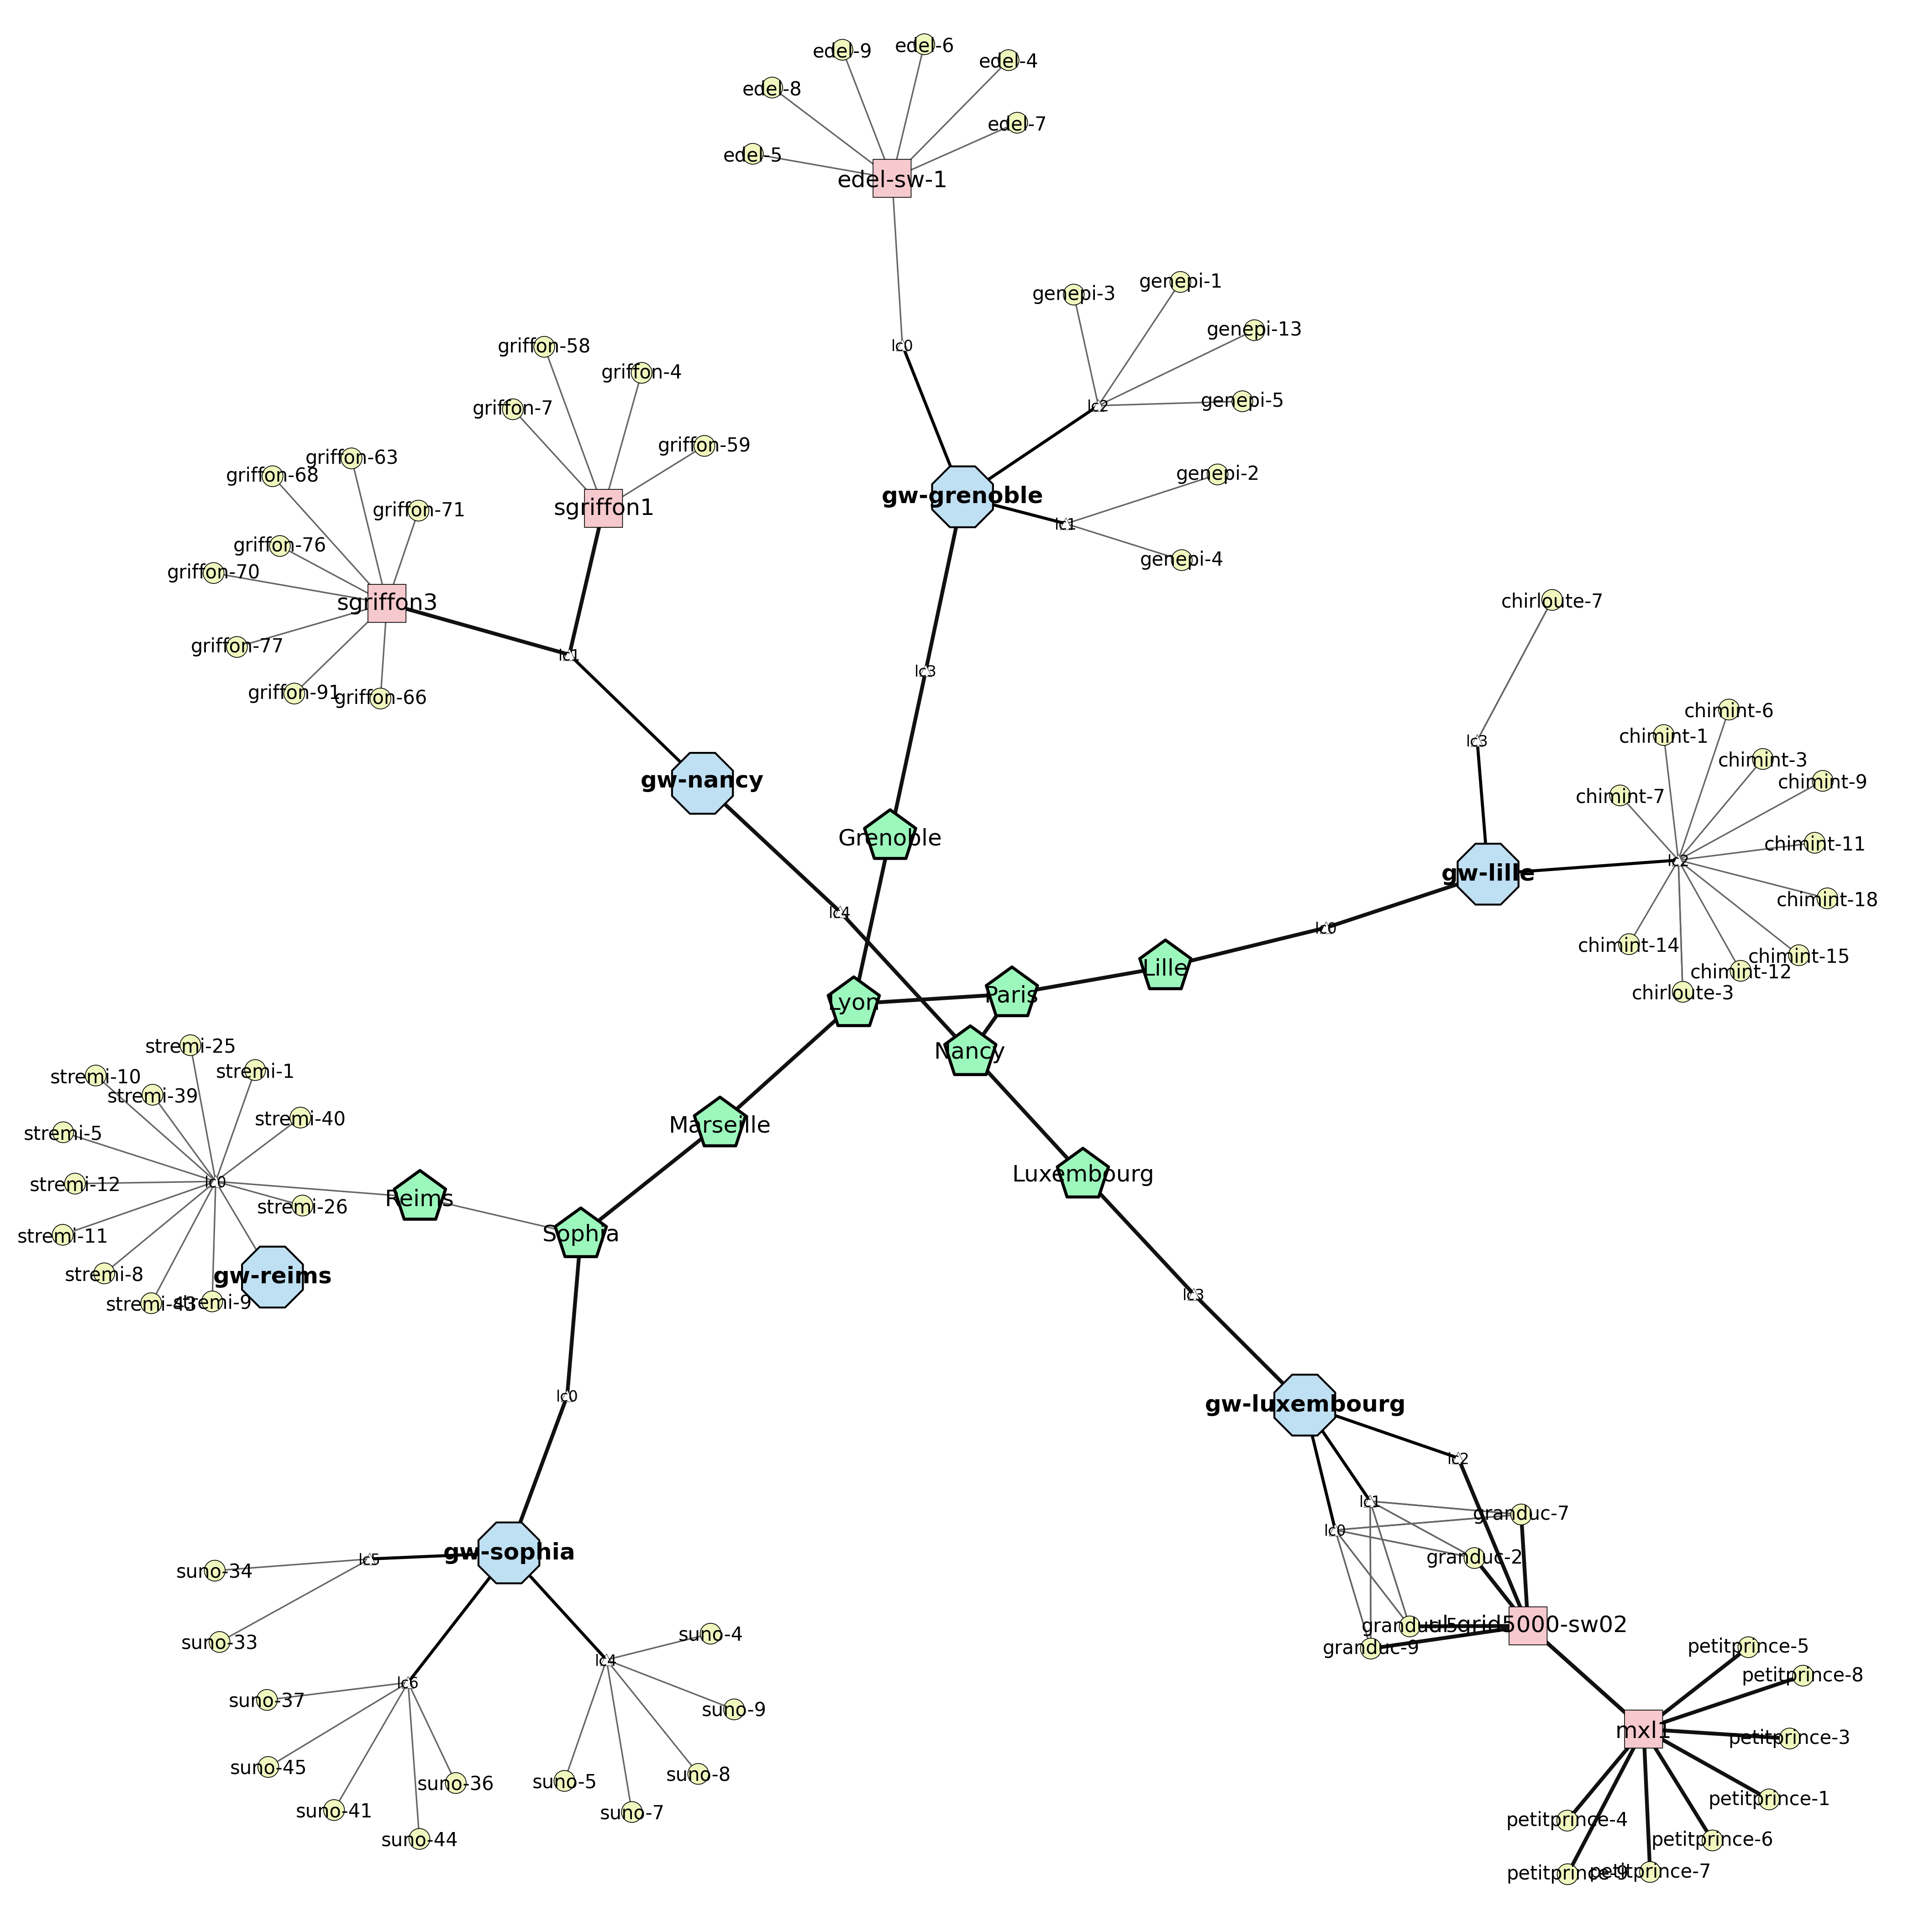
\includegraphics[width=7cm]{figures/6_sites.png}
%    \caption{Test-cases on the Grid'5000 platform involving 6
%    geographically-spreaded sites each hosting 2 controllers and 10 computes
%    nodes.}
%\end{figure}


%\subsubsection{Test-cases}
%\paragraph{Monosite}
%\paragraph{Multisite: 1 controller per site}
%\paragraph{Multisite: 10 controllers per site}
